%!TEX root = ../MasterThesis.tex

\section{Building a partially centralized \gls{P2P} system}
\label{sec:p2p_partially_centralized_system}

For the \gls{E-commerce} fraud scenario, that has been selected for this thesis in Section~\ref{sec:scope_thesis}, one can say that the issuer of a credit card is the party who initiates the collaborative fraud investigation. They are recognizing the active use (and likely misuse) of a credit card in the online and the offline world first, and are also getting a notification about any suspicious transactions made with it from their fraud prevention systems. Due to this fact, one can come up with a partially centralized \gls{P2P} architecture for the \gls{E-commerce} fraud investigation system, in that the issuer of a card in at the center and acts as a trusted party in this system. This issuer will initiate a collaborative session with the other required stakeholders based on the usage history of the credit card in question. During this \gls{P2P} communication session the merchants, \gls{PSP}s and \gls{LSP}s will share the required information with the issuer. In this process the data from the other stakeholders will be replicated to the issuer, who will build up a networked graph based on the Schema.org specification. So the main work will be on the issuer's side, who is the major driving party in the system, as depicted in Figure~\ref{fig:images_p2p_centralized}.\@

\begin{figure}[H]
	\centering
		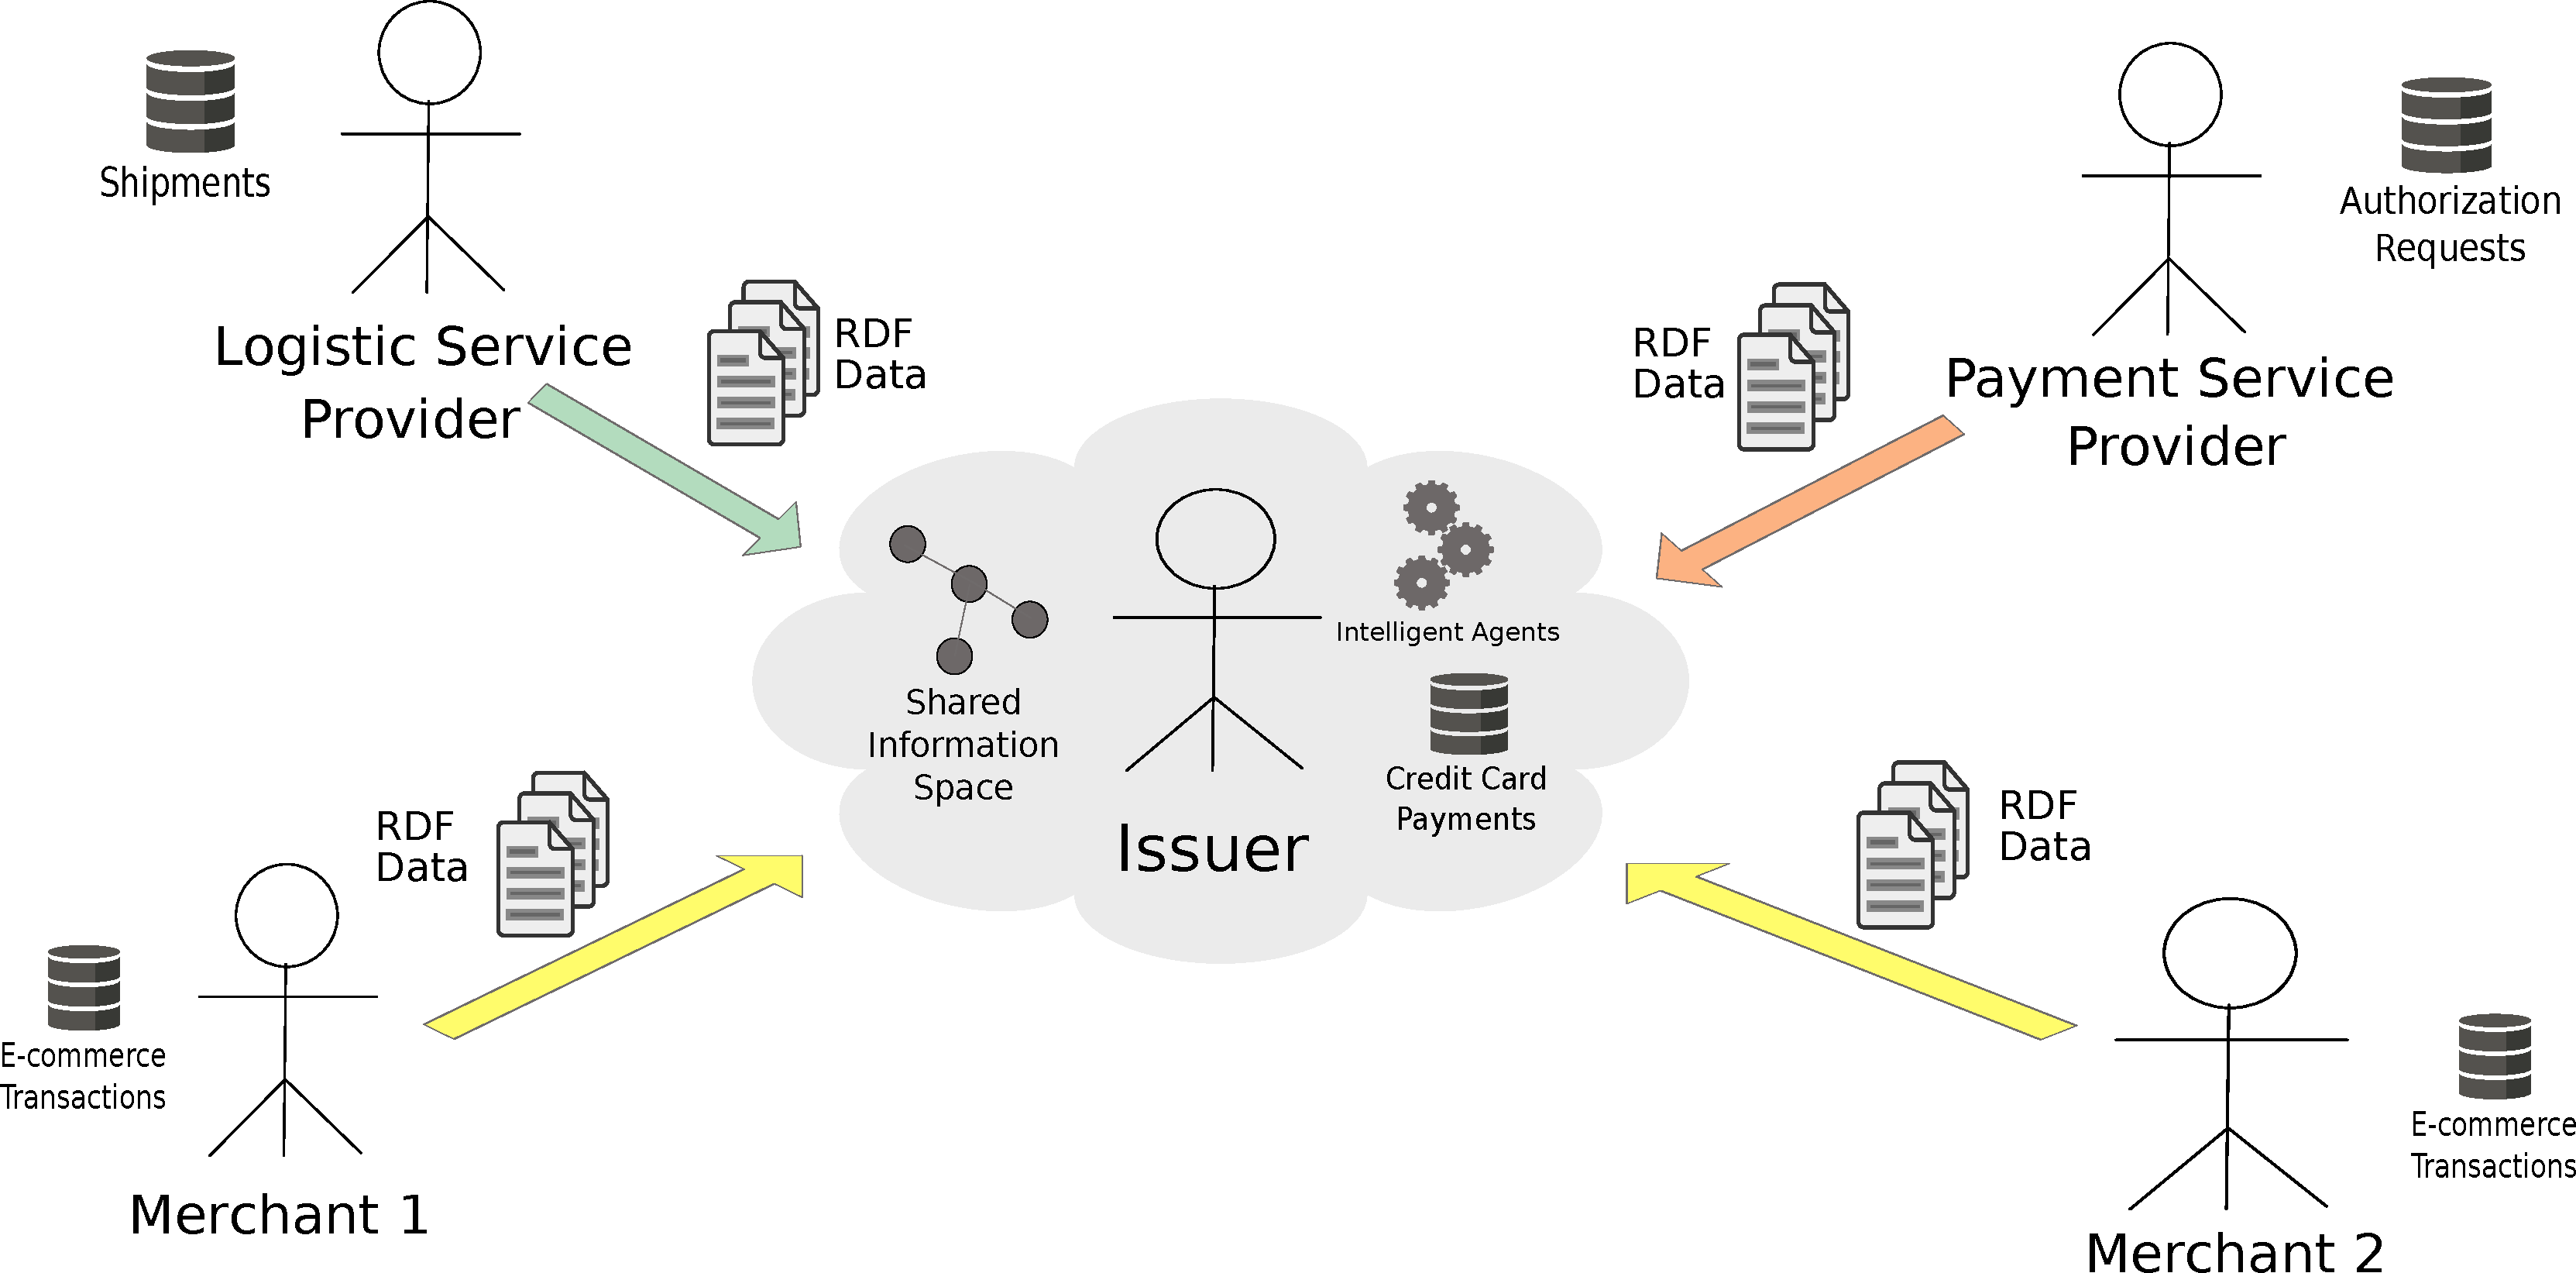
\includegraphics[width=0.9\columnwidth]{images/system_P2P_centralized.pdf}
	\caption{Collaborative system using a partially centralized \gls{P2P} architecture}
\label{fig:images_p2p_centralized}
\end{figure}

Using the \gls{WebRTC} communication protocol for initiating the \gls{P2P} session will allow the issuers to setup a communication between the relevant stakeholders directly from within an application running in their Web browsers. The application can visualize the connectivity status of the participants, the progress of their data sharing efforts as well as offer direct face-to-face communication possibilities in case of misunderstandings or further requests. \\

One of the major issues with the above mentioned system architecture is, that the merchants, \gls{PSP}s and \gls{LSP}s have to hand over all of their relevant information to the issuer of a credit card for the analysis. \\

\ldots

% subsec p2p_partially_centralized_system

% section design_proposal (end)
